\textcolor{secundario}{ENFOQUE DE INGRESOS. M\'etodo de valuaci\'on por capitalizaci\'on directa. }\\



Una \textcolor{principal}{perpetuidad} es una serie de flujos de caja infinita en el tiempo. \\

Las \textcolor{principal}{perpetuidades} son similares a las anualidades en el sentido que son pagos por montos iguales realizados en intervalos de tiempo iguales, la diferencia es que los pagos o cuotas de las perpetuidades son para siempre, tal y como su nombre indica. \\

Esta herramienta es especialmente \'util para valuar empresas y, por ende, sus acciones, dada su naturaleza de tener vida perpetua. Algunas inversiones, como las acciones preferentes y bonos, son perpetuidades en esencia, y para transferir estos activos de los inversores a los inversionistas es necesario que cuenten con un valor presente.\\

La perpetuidad puede ser simple, si los flujos de caja son constantes en el tiempo, o creciente, si \'estos son cada vez mayores:\\


\begin{center}
\begin{figure}[H]
\centering
	\caption{Capitalizaci\'on Directa mediante perpetuidad creciente\label{fig:cap_dir}}
	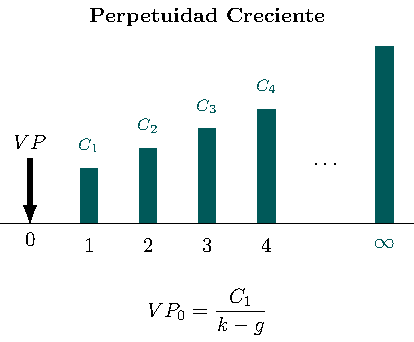
\includegraphics[width=5cm]{\rutaImagenes/capitalizacion_directa}\\
	
	\begin{minipage}{5cm}
	Donde:
	\begin{itemize}
	
		\item $C_1$: Flujo de caja
		\item $k$: Tasa de Capitalizaci\'on
		\item $g$: Tasa de Crecimiento
	\end{itemize}
	\end{minipage}
\end{figure}
\end{center}

\textcolor{principal}{Capitalizaci\'on mediante una perpetuidad creciente.} Se refiere al caso en la que el valor de un flujo de ingresos demuestra una tendencia notable al alza y constante durante per\'iodos anuales sucesivos. En t\'erminos de inversiones, \'esto a menudo se traduce en una situaci\'on en la que el rendimiento anual anticipado de la inversi\'on se alcanza de manera constante e incluso se excede de un a\~no al siguiente. El concepto tambi\'en implica que este flujo de efectivo continuar\'a en el futuro previsible, si el inversor elige conservar el activo durante un periodo de muchos a\~nos.\\


La evaluaci\'on del potencial para una perpetuidad creciente es a menudo muy importante para los inversores que desean adquirir una inversi\'on determinada con el objetivo de mantener esa inversi\'on durante varios a\~nos. Parte del proceso de evaluar con precisi\'on la presencia de una perpetuidad creciente de a\~no en a\~no implica tener en cuenta los cambios en el estado general de la econom\'ia. Esto significa que puede ser necesario ajustar las cifras de un a\~no determinado para compensar el efecto de la inflaci\'on. \\[10pt]

